\begin{frame}
    \frametitle{Постановка классификации}
        \small
        Пользовательские классы заранее неизвестны:
        \[
            Y_{\text{user}}=\{y_1,\dots,y_K\}.
        \]
        Если уверенного решения нет, система возвращает служебный исход
        \texttt{other}:
        \[
            \widetilde{Y}=Y_{\text{user}}\cup\{\texttt{other}\}.
        \]
        \[
            f(x)=
            \begin{cases}
                y_{k^*}, & \max_k s_k(x)\geqslant\tau,\\
                \texttt{other}, & \max_k s_k(x)<\tau.
            \end{cases}
        \]
\end{frame}

\section{Проектирование системы}

\begin{frame}
    \frametitle{Архитектура приложения}
    \centering
    \resizebox{0.98\linewidth}{!}{\begin{tikzpicture}[
        thick,
        >=stealth,
        node distance=6mm and 7mm,
        mod/.style={
                draw,
                rounded corners=2pt,
                align=center,
                minimum height=12mm,
                minimum width=24mm,
                inner sep=3pt,
                font=\small,
            },
        ctrl/.style={
                draw,
                rounded corners=2pt,
                align=center,
                minimum height=9mm,
                minimum width=40mm,
                inner sep=3pt,
                font=\small,
                fill=black!4,
            },
        store/.style={
                draw,
                rounded corners=2pt,
                align=center,
                minimum height=11mm,
                inner sep=3pt,
                font=\small,
                fill=black!4,
            },
    ]
    \node[ctrl]                                            (orch)  {orchestration\\(управление процессом)};
    \node[ctrl, below=of orch]                             (queue) {queueing\\очередь \texttt{pipeline\_tasks}};

    \node[mod, below=12mm of queue.south, anchor=north, xshift=-52mm] (email) {email\\синхронизация,\\нормализация};
    \node[mod, right=of email]                             (clu)   {clustering\\эмбеддинги,\\HDBSCAN / KMeans};
    \node[mod, right=of clu]                               (ann)   {annotation\\Argilla:\\экспорт / импорт};
    \node[mod, right=of ann]                               (clf)   {classifier\\прототипы,\\порог};
    \node[mod, right=of clf]                               (eval)  {evaluation\\метрики,\\дрейф};

    \node[store, below=12mm of email.south west, anchor=north west, minimum width=147mm]
                                                           (store) {storage "--- PostgreSQL\\(письма, нормализованные тексты, эмбеддинги, кластеры, метки, прототипы)};

    \draw[->] (orch) -- (queue);
    \draw[->] (email) -- (clu);
    \draw[->] (clu)   -- (ann);
    \draw[->] (ann)   -- (clf);
    \draw[->] (clf)   -- (eval);

    \draw[->] (queue.south) -| (email.north);
    \draw[->] (queue.south) -| (clf.north);

    \draw[<->, dashed] (email) -- (email |- store.north);
    \draw[<->, dashed] (clu)   -- (clu   |- store.north);
    \draw[<->, dashed] (ann)   -- (ann   |- store.north);
    \draw[<->, dashed] (clf)   -- (clf   |- store.north);
    \draw[<->, dashed] (eval)  -- (eval  |- store.north);
\end{tikzpicture}
}

    \medskip
    \small
    Обработка выполняется локально: IMAP-синхронизация только на~чтение,
    PostgreSQL для трассируемого хранения, очередь задач для повторяемого
    исполнения этапов.
\end{frame}

\begin{frame}
    \frametitle{Данные и экспериментальная установка}
    \centering
    \small
    \begin{tabular}{@{}ll@{}}
        \toprule
        Характеристика & Значение \\
        \midrule
        Всего писем после синхронизации & 7107 \\
        Писем для построения эмбеддингов & 7105 \\
        Доля русскоязычных / англоязычных писем & 0{,}91 / 0{,}09 \\
        Период & 03.2012--05.2026 \\
        \bottomrule
    \end{tabular}

    \medskip
    \begin{itemize}
        \item эмбеддинги: \texttt{BAAI/bge-m3}, 1024 измерения;
        \item разметка и~оценка: 1000 наиболее свежих писем;
        \item разбиение: 70\,\% обучение, 30\,\% тест;
        \item начальное значение генератора: 42.
    \end{itemize}
\end{frame}

\section{Кластеризация и разметка}

\begin{frame}
    \frametitle{Эмбеддинги и кластеризация}
    \begin{columns}[T,onlytextwidth]
        \begin{column}{0.47\linewidth}
            \small
            \begin{itemize}
                \item Готовая модель \texttt{BAAI/bge-m3} из~библиотеки
                      sentence-transformers строит единое пространство
                      для~русских и~английских писем.
                \item Готовая библиотечная реализация HDBSCAN выделяет
                      плотные группы и~шумовые точки.
                \item Параметры \texttt{min\_cluster\_size} и
                      \texttt{min\_samples} подбираются оптимизацией
                      рандомным перебором с~закреплением лучшего варианта.
            \end{itemize}
        \end{column}
        \begin{column}{0.50\linewidth}
            \small
            Подбор параметров:
            \begin{itemize}
                \item проверено 100 наборов на~пакете из~200 писем;
                \item целевая функция учитывала DBCV и~долю шума;
                \item для эксперимента закреплены
                      \texttt{min\_cluster\_size}=8 и~\texttt{min\_samples}=3.
            \end{itemize}
        \end{column}
    \end{columns}
\end{frame}

\begin{frame}
    \frametitle{Результаты кластеризации}
    \begin{columns}[T,onlytextwidth]
        \begin{column}{0.50\linewidth}
            \centering
            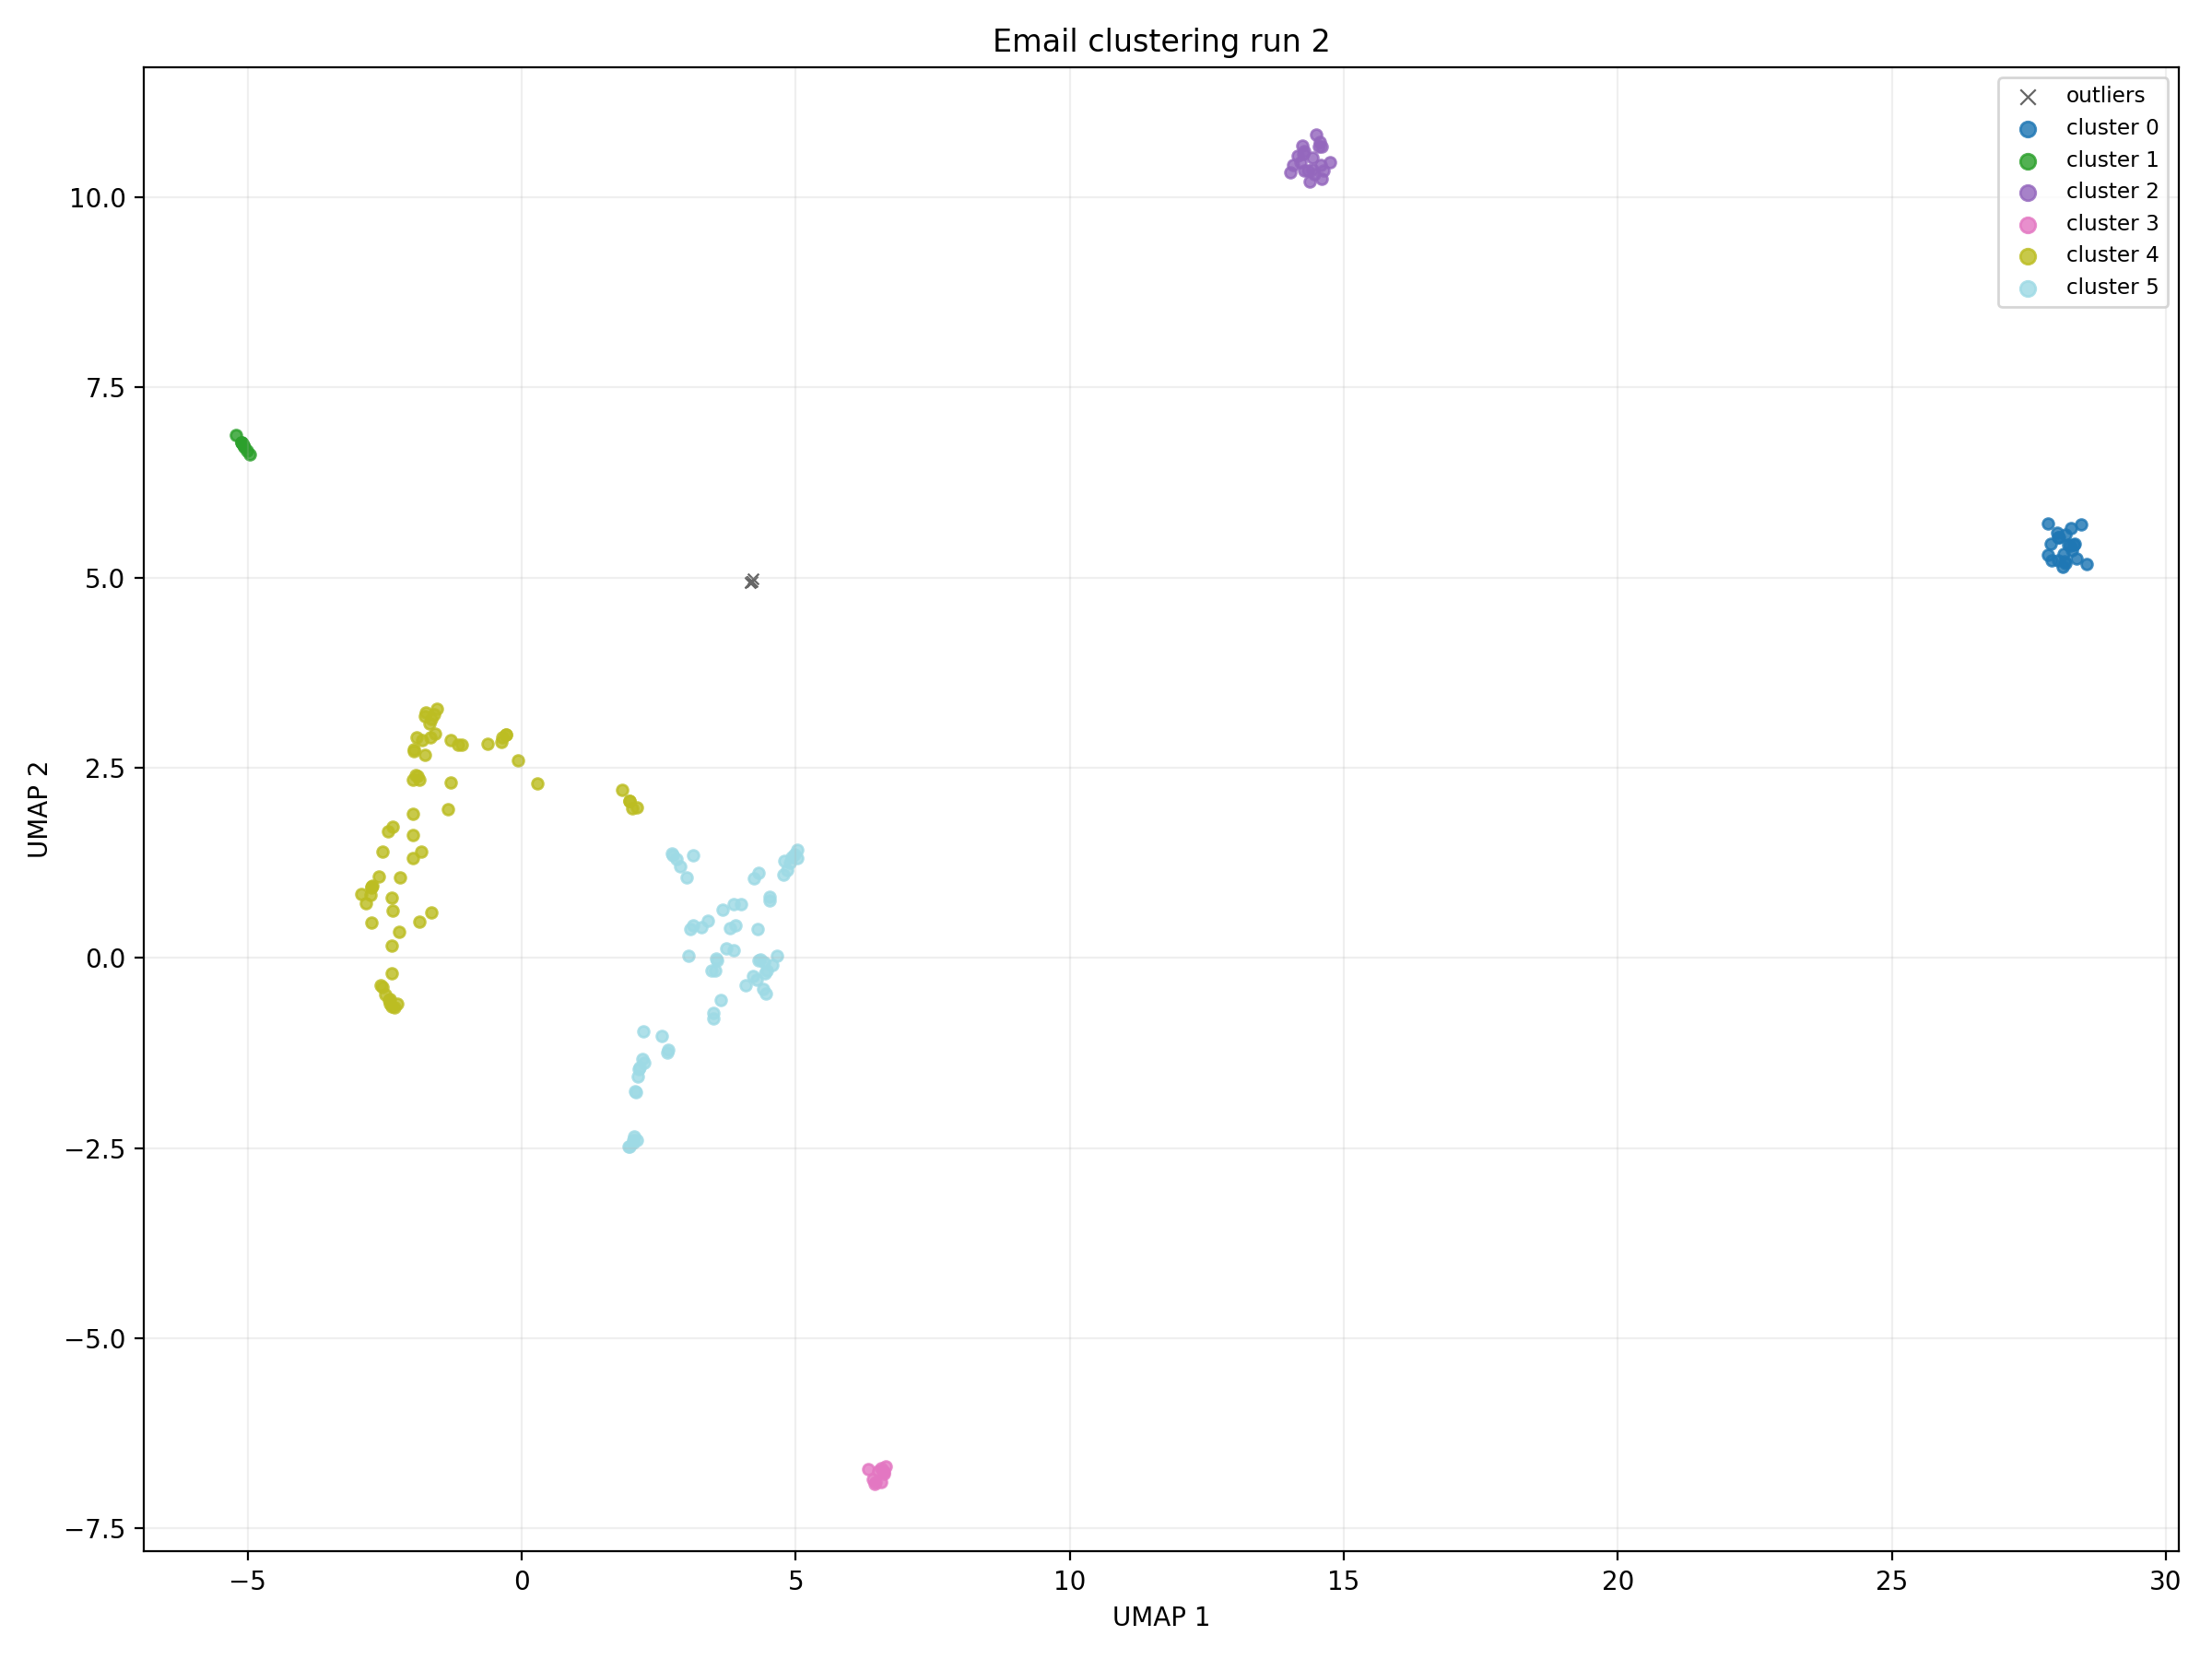
\includegraphics[width=\linewidth]{Dissertation/images/cluster_projection}
        \end{column}
        \begin{column}{0.47\linewidth}
            \scriptsize
            \begin{tabular}{@{}rrrrr@{}}
                \toprule
                Пакет & Кл. & Шум & Сил. & DBCV \\
                \midrule
                1 & 6  & 0{,}025 & 0{,}808 & 0{,}732 \\
                2 & 13 & 0{,}030 & 0{,}653 & 0{,}600 \\
                3 & 20 & 0{,}020 & 0{,}715 & 0{,}727 \\
                4 & 17 & 0{,}010 & 0{,}757 & 0{,}773 \\
                5 & 13 & 0{,}010 & 0{,}786 & 0{,}799 \\
                \midrule
                \(\Sigma\)/ср. & 69 & 0{,}019 & 0{,}744 & 0{,}726 \\
                \bottomrule
            \end{tabular}

            \medskip
            \small
            Пять пакетов по~200 писем дали 69 тематических кластеров при
            средней доле шума 1{,}9\,\%.
        \end{column}
    \end{columns}
\end{frame}

\begin{frame}
    \frametitle{Ручная проверка и сформированные классы}
    \begin{columns}[T,onlytextwidth]
        \begin{column}{0.47\linewidth}
            \small
            \begin{itemize}
                \item Проверка представителей кластеров
                      в~интерфейсе ручной разметки.
                \item Согласованная метка распространяется на~весь кластер.
                \item Противоречивые кластеры и~шум переходят в~\texttt{other}.
                \item Ручная проверка: 345 представителей из~1000 писем.
                \item Экономия ручной разметки: около 65{,}5\,\%.
            \end{itemize}
        \end{column}
        \begin{column}{0.50\linewidth}
            \scriptsize
            \begin{tabular}{@{}lr@{}}
                \toprule
                Класс & Число писем \\
                \midrule
                реклама & 296 \\
                безопасность & 208 \\
                apple & 114 \\
                подписки & 95 \\
                авторизация & 86 \\
                социальные сети & 47 \\
                todoist & 44 \\
                личные письма & 23 \\
                \texttt{other} & 87 \\
                \bottomrule
            \end{tabular}
        \end{column}
    \end{columns}
\end{frame}

\section{Классификация и оценка}

\begin{frame}
    \frametitle{Прототипный классификатор}
    \small
    Для каждого пользовательского класса строится один или несколько
    нормированных прототипов. Оценка класса равна максимальной косинусной
    близости письма к~его прототипам.

    \begin{columns}[T,onlytextwidth]
        \begin{column}{0.49\linewidth}
            \begin{itemize}
                \item \texttt{max\_per\_class} = 5;
                \item \texttt{min\_support\_per\_prototype} = 3;
                \item рабочий порог уверенности \(\tau=0{,}55\).
            \end{itemize}
        \end{column}
        \begin{column}{0.48\linewidth}
            \begin{block}{Причина выбора}
                Прототипная схема не~требует дообучения нейросети и~может
                применяться при ограниченном объёме проверенной разметки.
            \end{block}
        \end{column}
    \end{columns}
\end{frame}

\begin{frame}
    \frametitle{Качество классификации}
    \begin{columns}[T,onlytextwidth]
        \begin{column}{0.36\linewidth}
            \small
            \begin{tabular}{@{}lr@{}}
                \toprule
                Метрика & Значение \\
                \midrule
                Accuracy & 0{,}842 \\
                macro-F1 & 0{,}835 \\
                weighted-F1 & 0{,}847 \\
                Покрытие & 0{,}996 \\
                \texttt{other} & 0{,}004 \\
                \bottomrule
            \end{tabular}

            \medskip
            \small
            Тестовая часть: 273 письма, 8 пользовательских классов.
        \end{column}
        \begin{column}{0.61\linewidth}
            \centering
            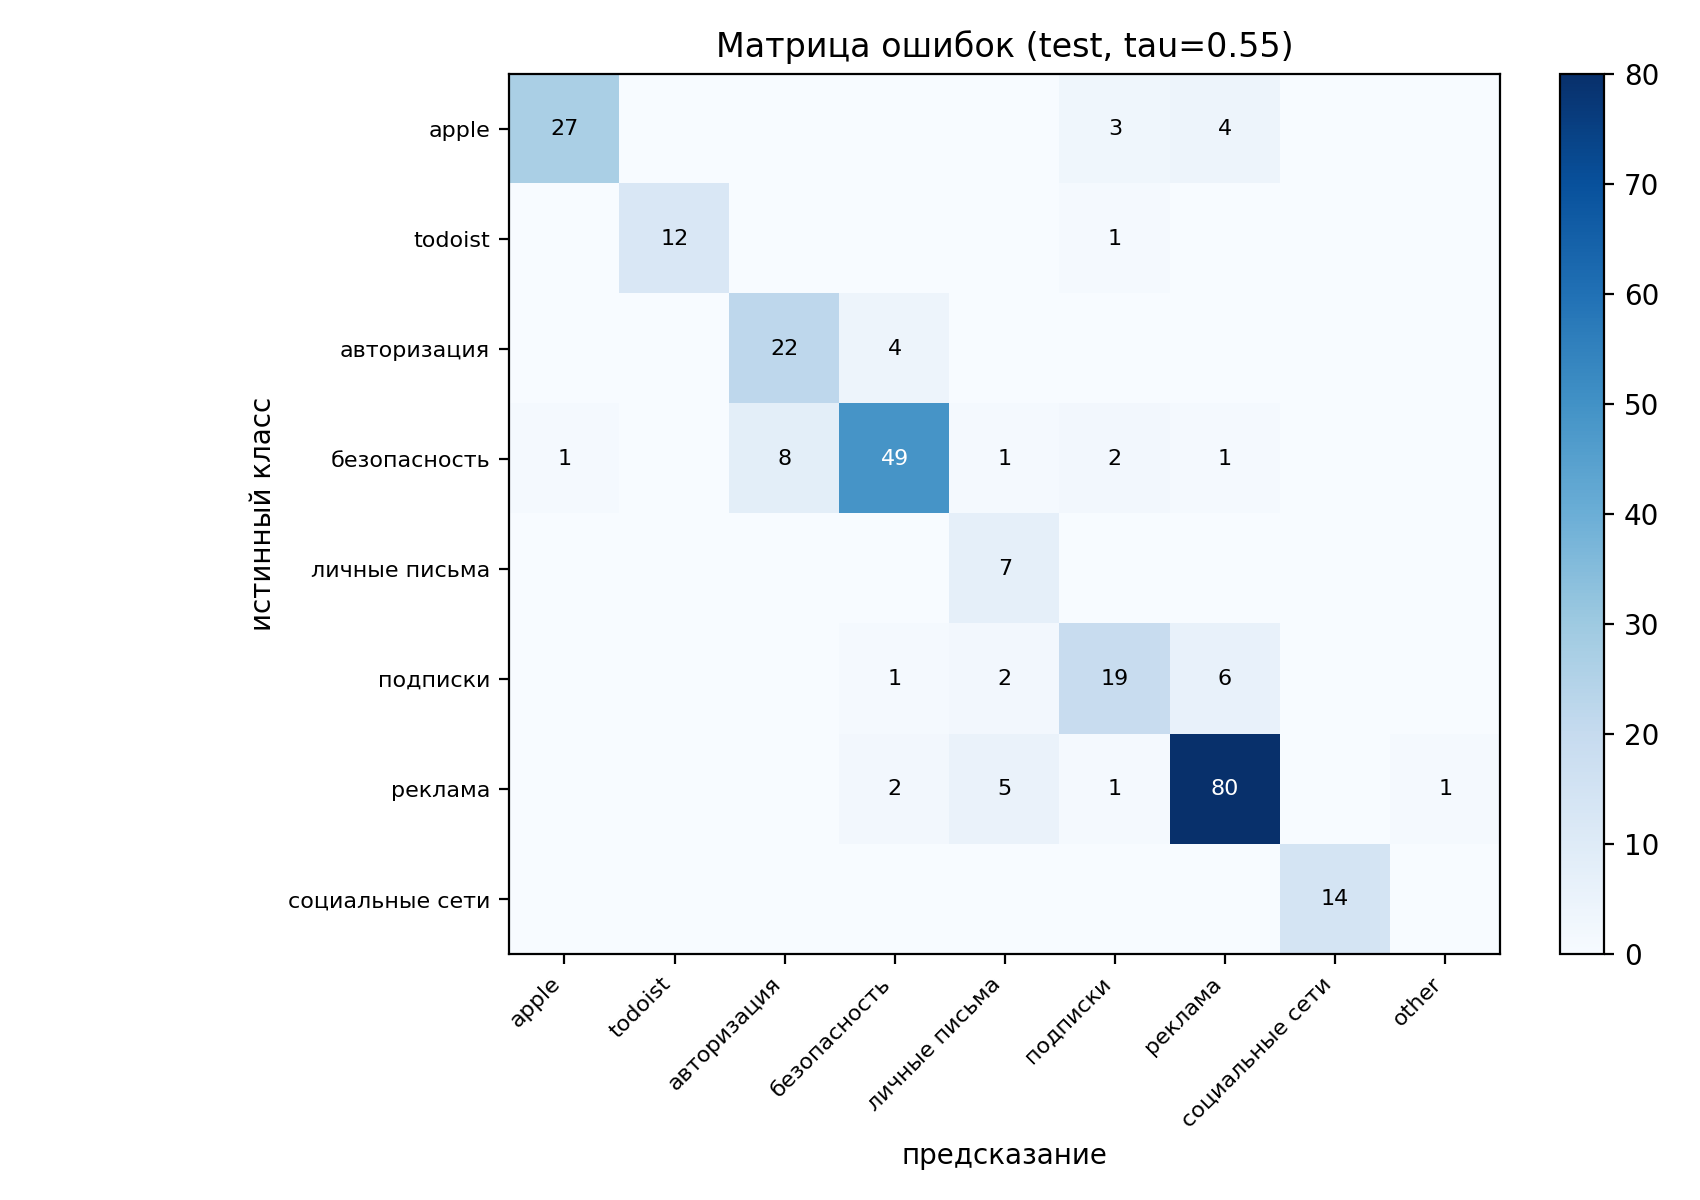
\includegraphics[width=\linewidth]{Dissertation/images/confusion_matrix}
        \end{column}
    \end{columns}
\end{frame}

\begin{frame}
    \frametitle{Порог уверенности и обновление модели}
    \begin{columns}[T,onlytextwidth]
        \begin{column}{0.52\linewidth}
            \centering
            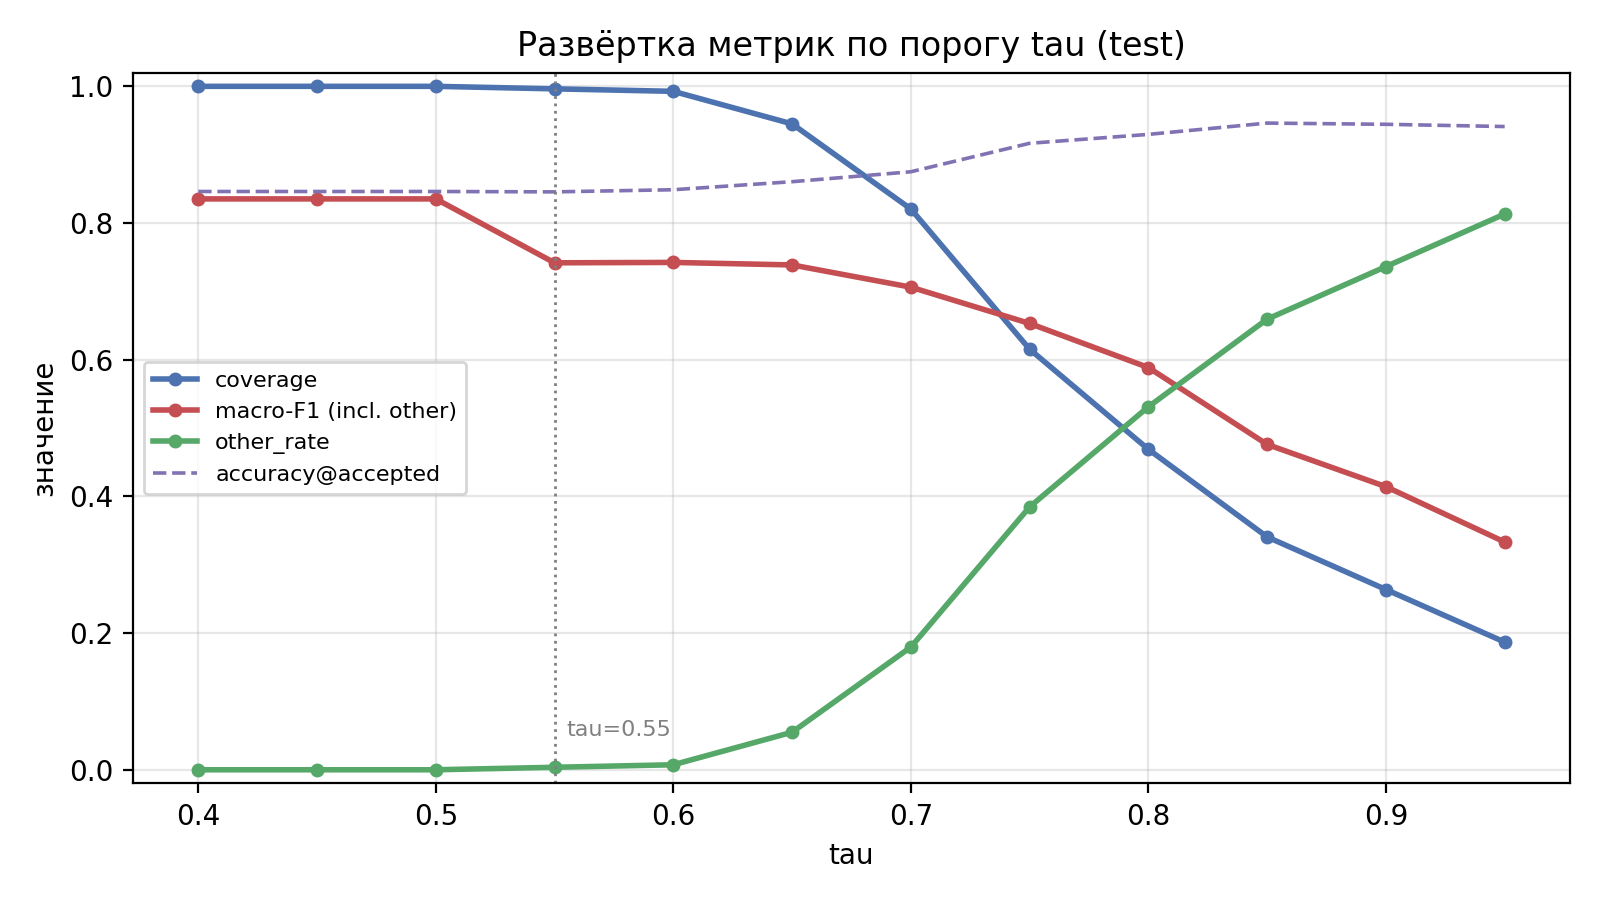
\includegraphics[width=\linewidth]{Dissertation/images/tau_sweep}
        \end{column}
        \begin{column}{0.45\linewidth}
            \small
            \begin{itemize}
                \item Повышение \(\tau\) увеличивает долю отказов
                      \texttt{other}.
                \item При \(\tau=0{,}55\) достигается покрытие 0{,}996
                      и~macro-F1 0{,}835 по~пользовательским классам.
                \item Буфер \texttt{other} служит источником новых данных
                      для следующего цикла разметки.
                \item В~первом прогоне буфер содержал 87 писем, что ниже
                      порога запуска нового цикла.
            \end{itemize}
        \end{column}
    \end{columns}
\end{frame}
